% mnras_template.tex 
%
% LaTeX template for creating an MNRAS paper
%
% v3.3 released April 2024
% (version numbers match those of mnras.cls)
%
% Copyright (C) Royal Astronomical Society 2015
% Authors:
% Keith T. Smith (Royal Astronomical Society)

% Change log
%
% v3.3 April 2024
%   Updated \pubyear to print the current year automatically
% v3.2 July 2023
%	Updated guidance on use of amssymb package
% v3.0 May 2015
%    Renamed to match the new package name
%    Version number matches mnras.cls
%    A few minor tweaks to wording
% v1.0 September 2013
%    Beta testing only - never publicly released
%    First version: a simple (ish) template for creating an MNRAS paper

%%%%%%%%%%%%%%%%%%%%%%%%%%%%%%%%%%%%%%%%%%%%%%%%%%
% Basic setup. Most papers should leave these options alone.
\documentclass[fleqn,usenatbib]{mnras}

% MNRAS is set in Times font. If you don't have this installed (most LaTeX
% installations will be fine) or prefer the old Computer Modern fonts, comment
% out the following line
\usepackage{newtxtext,newtxmath}
% Depending on your LaTeX fonts installation, you might get better results with one of these:
%\usepackage{mathptmx}
%\usepackage{txfonts}

% Use vector fonts, so it zooms properly in on-screen viewing software
% Don't change these lines unless you know what you are doing
\usepackage[T1]{fontenc}

% Allow "Thomas van Noord" and "Simon de Laguarde" and alike to be sorted by "N" and "L" etc. in the bibliography.
% Write the name in the bibliography as "\VAN{Noord}{Van}{van} Noord, Thomas"
\DeclareRobustCommand{\VAN}[3]{#2}
\let\VANthebibliography\thebibliography
\def\thebibliography{\DeclareRobustCommand{\VAN}[3]{##3}\VANthebibliography}


%%%%% AUTHORS - PLACE YOUR OWN PACKAGES HERE %%%%%

% Only include extra packages if you really need them. Avoid using amssymb if newtxmath is enabled, as these packages can cause conflicts. newtxmatch covers the same math symbols while producing a consistent Times New Roman font. Common packages are:
\usepackage{graphicx}	% Including figure files
\usepackage{amsmath}	% Advanced maths commands

%%%%%%%%%%%%%%%%%%%%%%%%%%%%%%%%%%%%%%%%%%%%%%%%%%

%%%%% AUTHORS - PLACE YOUR OWN COMMANDS HERE %%%%%

% Please keep new commands to a minimum, and use \newcommand not \def to avoid
% overwriting existing commands. Example:
%\newcommand{\pcm}{\,cm$^{-2}$}	% per cm-squared

%%%%%%%%%%%%%%%%%%%%%%%%%%%%%%%%%%%%%%%%%%%%%%%%%%

%%%%%%%%%%%%%%%%%%% TITLE PAGE %%%%%%%%%%%%%%%%%%%

% Title of the paper, and the short title which is used in the headers.
% Keep the title short and informative.
\title[Research Assignment 2]{Research Assignment 2: Proposal}

% The list of authors, and the short list which is used in the headers.
% If you need two or more lines of authors, add an extra line using \newauthor
\author[E. H. S. Figureido]{Ethan H. S. Figureido$^{1}$}


% Prints the current year, for the copyright statements etc. To achieve a fixed year, replace the expression with a number. 
\pubyear{\the\year{}}

% Don't change these lines
\begin{document}
\label{firstpage}
\pagerange{\pageref{firstpage}--\pageref{lastpage}}
\maketitle

%%%%%%%%%%%%%%%%%%%%%%%%%%%%%%%%%%%%%%%%%%%%%%%%%%

%%%%%%%%%%%%%%%%% BODY OF PAPER %%%%%%%%%%%%%%%%%%

\section{Introduction}

A majority of the matter in the universe takes the form of dark matter: a collisionless particle that doesn't emit radiation, and interacts only gravitationally with other matter. Dark matter clusters into filaments that form halos where they intersect. These halos are the sites of galaxy formation, and they have great influence on the structure and dynamics of the galaxies they encompass, determining their evolution. 

As they are the sites of galaxy formation and evolution, their properties are linked to the evolutionary history and properties of galaxies. The structure of these halos in particular is key to understanding galaxy formation and evolution. Understanding how different environments produce different halo structures will provide insight into galaxy merger histories \citep{Drakos_2019}. For example, the shape of a halo is connected to the previous major merger, being stretched along the merger axis \citep{Despali_2016}. Understanding what environments different shapes emerge in will help us understand galaxy merger histories, and may make them a powerful indicator of a galaxy's merger history.

Our understanding of galaxy evolution has been crafted by galaxy modeling and observation; observation acting to refine the constraints of our simulations. From this, we have learned much about the relationship between dark matter halos and the baryonic matter within them. Dark matter halos grow through accretion of surrounding matter, and mergers. This growth is anisotropic, and will create triaxial and prolate halo shapes in isolation. Baryonic processes like black hole feedback, radiative processes, and star formation work to smooth the shape of the halo, giving it an oblate shape. Fig.3 from \citet{Prada_2019} illustrates the effects of baryonic processes on halo shape by comparing the axes ratios of halos from magneto-hydrodynamic simulations, which include baryonic effects, and dark matter only simulations which don't. These simulations provide insight into how halos are shaped by the baryonic matter that they encompass. 

\begin{figure}
	\includegraphics[width=\columnwidth]{fig 3 prada+2019.jpg}
    \caption{Figure 3 from \citet{Prada_2019}. Plotting the axes ratios for 30 simulated dark matter halos for dark matter only (DMO, left) and magneto-hydrodynamic (MHD, right) simulations. Triangles indicate data for the inner regions (R200/16 (~14kpc)) of the halos. They visualize three main population trends: DMO simulations are rounder in the outer regions than the inner, MHD simulations are rounder in the inner regions than the outer, and MHD halos are rounder than DMO halos}
    \label{fig:MHD vs DMO}
\end{figure}

Much of the uncertainty surrounding this topic stems from the variety of methods used and inadequate resolution. Further, the exact effects of baryons on dark matter haloes is still being hashed out. The differing environments, and the assumptions and uncertainties of different simulations has produced evidence favoring all possible halo configurations, as discussed in \citet{Chua_2019} and \citet{Prada_2019}. Many of the open questions surround the reliability of observations and assumptions used to constrain simulations.


%%%%%%%%%%%%%%%%%%%%%%%%%%%%%%%%%%%%
\section{Proposal}

The following is the proposal for a study of the shape and evolution of the MW-M31 merger dark matter remnant using data from the simulation found in the \citet{van_der_Marel_2012} study.

%%%%%%%%%%%%%%%%%%%%%%%%%%%%%%%%%%%%%%
\subsection{This Proposal}

Using the MW-M31-M33 simulation data, I aim to determine if the shape of the combined dark matter halo of the MW-M31 merger is oblate, prolate, or triaxial, and discuss how it evolves over time.

%%%%%%%%%%%%%%%%%%%%%%%%%%%%%%%%%%%%%%
\subsection{Methods}

Dark matter halos take four main shapes: spherical, oblate, prolate, and triaxial. In a galactocentric reference frame an oblate spheroid is a sphere stretched along its y-axis, giving it a grapefruit shape, and a prolate spheroid is a sphere stretched along its z-axis, giving it an American football shape. A triaxial shape has different lengths for all three of its axes.

To answer the question of merged halo shape, we must determine when the MW-M31 merger is completed in the simulation, combine the halo particle data of both galaxies, and determine the edge of the dark matter halo before we can analyze the data.

A galaxy merger is considered complete when there is only one discernible center of mass (COM). Using the OrbitCOM code from homework 6, we can determine the snapshot where the merger is complete. By graphing the separation of the COM of the MW and M31, we can identify the snapshot where the separation of their COM is approximately zero (or oscillates closely about zero), implying a completed merger, as seen in Fig.~\ref{fig:COM separation}. From here, we can combine the MW and M31 halo particle arrays to get a complete set of particles for the merged halo.


\begin{figure}
	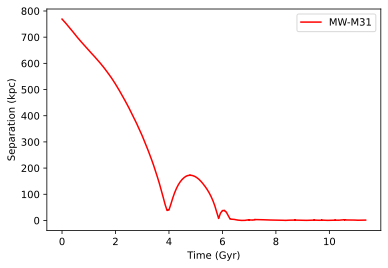
\includegraphics[width=\columnwidth]{MW-M31 Separation.png}
    \caption{Graph of COM separation for the MW and M31. The separation drops to zero at approximately 6.3 Gyr, slightly larger than the value found in \citet{van_der_Marel_2012} of 5.86 Gyr.}
    \label{fig:COM separation}
\end{figure}

Using the splashback radius, the radius where particles reach the apocenter of their first orbit, we can determine the edge of our halo. Of the three definitions of the halo edge (Rvir, R200, and the splashback radius), the splashback radius tends to be the largest, to our benefit. After a chaotic merger of two massive galaxies, particles are scattered to large radii. Including these particles is essential to understanding how the shape of the dark matter halo changes overtime, as these particles fall into the denser regions of the halo. 

From here we will plot the particle positions to visualize and interpret the shape of the halo. Plotting cross sections along the xy, xz, and yz planes will help fit ellipses to each spatial plane and determine ellipticity values. Making a 3D-plot of the outer edges of the halo will also help with visualization. These plots can be made for each snapshot. Using the data from each, it is possible to create an animation that we can analyze to determine how the shape is altered over time. 

%%%%%%%%%%%%%%%%%%%%%%%%%%%%%%%%%%%%%%
\subsection{Hypothesis}

From \citet{Despali_2016} a shape elongated along the merger axis is expected. Radiative processes, star formation, and AGN feedback are absent in this simulation. These processes generally smooth the halo to create a more oblate shape, so the simulation is expected to favor a non-oblate shape. Further, because these halos are so large, we expect the growth of the halo to begin with an initially triaxial shape. Combining the above, a triaxial halo with its longest axis in the direction of the merger axis is expected as the merged halo shape.


%%%%%%%%%%%%%%%%%%%% REFERENCES %%%%%%%%%%%%%%%%%%

% The best way to enter references is to use BibTeX:

\bibliographystyle{mnras}
\bibliography{example} % if your bibtex file is called example.bib


% Alternatively you could enter them by hand, like this:
% This method is tedious and prone to error if you have lots of references
%\begin{thebibliography}{99}
%\bibitem[\protect\citeauthoryear{Author}{2012}]{Author2012}
%Author A.~N., 2013, Journal of Improbable Astronomy, 1, 1
%\bibitem[\protect\citeauthoryear{Others}{2013}]{Others2013}
%Others S., 2012, Journal of Interesting Stuff, 17, 198
%\end{thebibliography}

%%%%%%%%%%%%%%%%%%%%%%%%%%%%%%%%%%%%%%%%%%%%%%%%%%


% Don't change these lines
\bsp	% typesetting comment
\label{lastpage}
\end{document}

% End of mnras_template.tex
